\documentclass[10pt,twocolumn,letterpaper]{article}

\usepackage[top=2.0cm,bottom=2.0cm,left=1.75cm,right=1.75cm]{geometry}
\usepackage{times}
\usepackage{amsmath,amssymb}
\usepackage{graphicx}
\usepackage{booktabs}
% \usepackage{microtype} % Disabled to accelerate Overleaf compile time
\usepackage{url}
\usepackage{xurl}
\usepackage[colorlinks=true,citecolor=blue,linkcolor=blue,urlcolor=blue]{hyperref}
\usepackage{subcaption}
\usepackage{indentfirst}
\usepackage{titlesec}
\usepackage[font=small,labelfont={bf},labelsep=period]{caption}

\graphicspath{{figures/}}

% Relax LaTeX float placement parameters to prevent float buffering and compile timeouts
\renewcommand{\topfraction}{0.95}
\renewcommand{\bottomfraction}{0.95}
\renewcommand{\textfraction}{0.05}
\renewcommand{\floatpagefraction}{0.85}
\renewcommand{\dbltopfraction}{0.95}
\renewcommand{\dblfloatpagefraction}{0.85}
\setcounter{topnumber}{4}
\setcounter{bottomnumber}{4}
\setcounter{totalnumber}{6}
\setcounter{dbltopnumber}{4}
\raggedbottom

% IEEE Style Section/Subsection Numbering
\renewcommand{\thesection}{\Roman{section}}
\renewcommand{\thesubsection}{\Alph{subsection}}

% Section Formatting: Tight, cohesive academic style
\titleformat{\section}
  {\normalsize\bfseries\scshape}
  {\thesection.}
  {0.5em}
  {}
\titlespacing*{\section}
  {0pt}
  {8pt plus 2pt minus 1pt}
  {3pt plus 1pt minus 1pt}

\titleformat{\subsection}
  {\normalsize\bfseries\itshape}
  {\thesubsection.}
  {0.5em}
  {}
\titlespacing*{\subsection}
  {0pt}
  {6pt plus 2pt minus 1pt}
  {2pt plus 1pt minus 1pt}

% Paragraph Formatting: Standard academic indentation, no vertical paragraph gaps
\setlength{\parindent}{14pt}
\setlength{\parskip}{0pt}

% Compact Math Display Spacing
\setlength{\abovedisplayskip}{3pt plus 1pt minus 1pt}
\setlength{\belowdisplayskip}{3pt plus 1pt minus 1pt}

\title{\Large \textbf{Automated Interpretation of Chest Radiographs: Decoupled Lesion Delineation, Multi-Scale Consensus Localization, and Structured Clinical Reporting}}

\author{
  \textbf{Dang J. Tuong}\\
  Faculty of Information Technology, Nam Can Tho University, Vietnam\\
  \texttt{tuongjdang@gmail.com}\\[2pt]
  \textit{Supervisor: M.Sc. Dang Manh Huy}
}
\date{}

\begin{document}
\maketitle

\begin{abstract}
Automated interpretation of chest radiographs involves detecting thoracic pathologies with fundamentally divergent spatial and morphological properties. Delicate boundary lesions, such as pneumothorax, necessitate pixel-accurate delineation to quantify visceral pleural displacement and lung collapse, whereas structural cardiac and mediastinal abnormalities are naturally characterized by bounding-box localization. Furthermore, clinical multi-reader datasets exhibit substantial inter-observer discordance and acute lesion scale bimodality, while conventional computer-aided systems fail to translate raw detections into standardized, actionable medical documentation. In this investigation, we establish an integrated clinical diagnostic system encompassing boundary segmentation, multi-scale consensus localization, and automated structured reporting. In the first phase, a U-Net++ architecture with an SE-ResNeXt-50 (32x4d) encoder and spatial/channel squeeze-and-excitation (scSE) attention is trained on the SIIM-ACR dataset under an asymmetric Focal-Tversky loss ($\beta=0.7$), yielding a Dice Similarity Coefficient of 84.42\% and an IoU of 82.21\% on 1,205 independent test radiographs. In the second phase, 14 pathological findings from the VinDr-CXR cohort are condensed into four clinical macro-classes and consolidated via Weighted Boxes Fusion (WBF), reducing inter-reader annotation noise by 46.7\%. To resolve the 66.1\% false-negative rate observed on micro-scale lesions ($<32\text{ px}$) by a single YOLOv11m baseline (mAP@50: 63.69\%), we formulate a multi-scale decoupled ensemble: Branch~A (YOLO11l @ 1024px) captures broad mediastinal context, while Branch~B (YOLO11m @ 1280px) quadruples pixel sampling for subtle opacities under anatomy-preserving training protocols ($\text{mosaic}=0.0$, $\text{flipud}=0.0$, $\text{mixup}=0.10$). Fused through grid-searched WBF ($\text{IoU}_{\text{thr}}=0.55$) and multi-scale test-time augmentation, the ensemble achieves an overall mAP@50 of \textbf{64.23\%} and elevates candidate recall to \textbf{90.07\%} (+27.04\% absolute gain). Finally, we implement an automated structured reporting engine that synthesizes predicted masks and consensus boxes into standardized radiological reports with quantitative geometric metrics, completing an end-to-end clinical workflow in 142.6~ms per image.
\end{abstract}

\noindent\textbf{Keywords:} Chest radiography, pneumothorax segmentation, U-Net++, YOLOv11, Weighted Boxes Fusion, Test-Time Augmentation, Multi-Model Ensemble, automated structured reporting, computer-aided diagnosis.

\section{Introduction}
Chest radiography represents the primary imaging modality for screening, triage, and diagnosing thoracic diseases worldwide. Despite its ubiquity, planar thoracic radiograph interpretation remains inherently challenging due to the projection of complex three-dimensional anatomical structures---ribs, clavicles, vascular trees, heart, and lung parenchyma---onto a single two-dimensional detector plane~\cite{litjens2017survey}. Superimposed tissue densities frequently obscure small pathologies or produce optical artifacts that mimic disease, inducing substantial cognitive fatigue and diagnostic variability among clinicians during emergency department triage and outpatient screening.

Clinical abnormalities on chest radiographs exhibit fundamentally distinct geometrical and morphological properties that cannot be handled optimally under a uniform single-architecture paradigm. Pneumothorax, for instance, manifests as a visceral pleural boundary separating the lung parenchyma from the chest wall, accompanied by peripheral radiolucency. Accurately assessing lung collapse and determining tube thoracostomy intervention requires pixel-accurate segmentation masks rather than rectangular bounding boxes~\cite{siim2019pneumothorax}. Conversely, structural cardiovascular conditions such as cardiomegaly and aortic enlargement occupy extensive, well-demarcated anatomical compartments where rectangular bounding boxes offer optimal diagnostic bounding and clinical alignment~\cite{nguyen2022vindrcxr}.

In addition to morphological divergence, clinical chest radiograph annotation suffers from notable inter-observer variability. In multi-reader clinical datasets, certified radiologists frequently disagree on the exact margins of diffuse opacities and effusions, producing overlapping annotations for the same pathological process. Standard Non-Maximum Suppression (NMS) arbitrarily discards overlapping boxes based solely on highest classification confidence, neglecting consensus information among expert annotators. Furthermore, empirical diagnostic analysis of lesion scale distributions reveals severe bimodality: while 95\% of cardiothoracic structural lesions are large ($>96\text{ px}$), over 21\% of pleural pathologies and 14\% of parenchymal opacities have micro-scale dimensions ($<32\text{ px}$). Under standard single-scale detectors ($640\times 640$), feature maps at deep network layers undergo spatial downsampling, causing subtle opacities to lose critical pixel representations.

To resolve these clinical and technical challenges, we investigate an integrated diagnostic framework that encompasses task-specific morphology, scale bimodality, and automated reporting. First, we develop a dedicated segmentation pipeline for pneumothorax on the SIIM-ACR cohort using U-Net++ with nested scSE attention and asymmetric loss penalties. Second, we restructure the VinDr-CXR cohort into four coherent clinical macro-classes and apply Weighted Boxes Fusion (WBF) to resolve reader discordance before training a YOLOv11m baseline. Third, to overcome the severe false-negative rate on small lesions, we construct a multi-scale specialist ensemble pairing a high-capacity model (YOLO11l @ 1024px) with an ultra-high-resolution model (YOLO11m @ 1280px) governed by anatomy-preserving data augmentations. Fourth, inference-time multi-scale Test-Time Augmentation (TTA) and single cardiac envelope post-processing are integrated to maximize lesion sensitivity. Finally, we formulate an automated structured reporting engine that extracts quantitative anatomical biomarkers---including the cardiothoracic ratio and pleural collapse fraction---and synthesizes standardized radiological documentation for emergency triage workflows.

\section{Materials and Dataset Curation}
\subsection{SIIM-ACR Pneumothorax Cohort}
The SIIM-ACR dataset~\cite{siim2019pneumothorax} comprises 12,047 high-resolution digital chest radiographs with pixel-level run-length encoded (RLE) masks annotated by board-certified radiologists. The dataset exhibits severe class imbalance, with only 22.1\% of cases demonstrating pneumothorax. We split the cohort into 9,637 training images (80\%), 1,205 validation images (10\%), and 1,205 held-out test images (10\%) using stratified sampling to guarantee identical disease distributions across all splits. Radiographs are resized to $512 \times 512$ resolution, and contrast is normalized using Contrast Limited Adaptive Histogram Equalization (CLAHE, clip limit 2.0, grid size $8\times 8$) to accentuate subtle pleural margins against background ribs.

\subsection{VinDr-CXR Abnormalities Cohort}
The VinDr-CXR cohort~\cite{nguyen2022vindrcxr} contains 15,000 retrospectively collected frontal chest radiographs independently annotated by 17 certified radiologists. Across the 67,914 raw annotation lines, substantial inter-observer discordance exists: 48.49\% of all annotated boxes share an overlap with an $\text{IoU} \ge 0.40$ with annotations from a peer radiologist. As shown in Figure~\ref{fig:curation}(a), annotations exhibit heavy concentration in cardiomegaly, aortic enlargement, and diffuse opacities alongside normal controls.

\begin{figure*}[!t]
  \centering
  \begin{subfigure}[b]{0.43\textwidth}
    \centering
    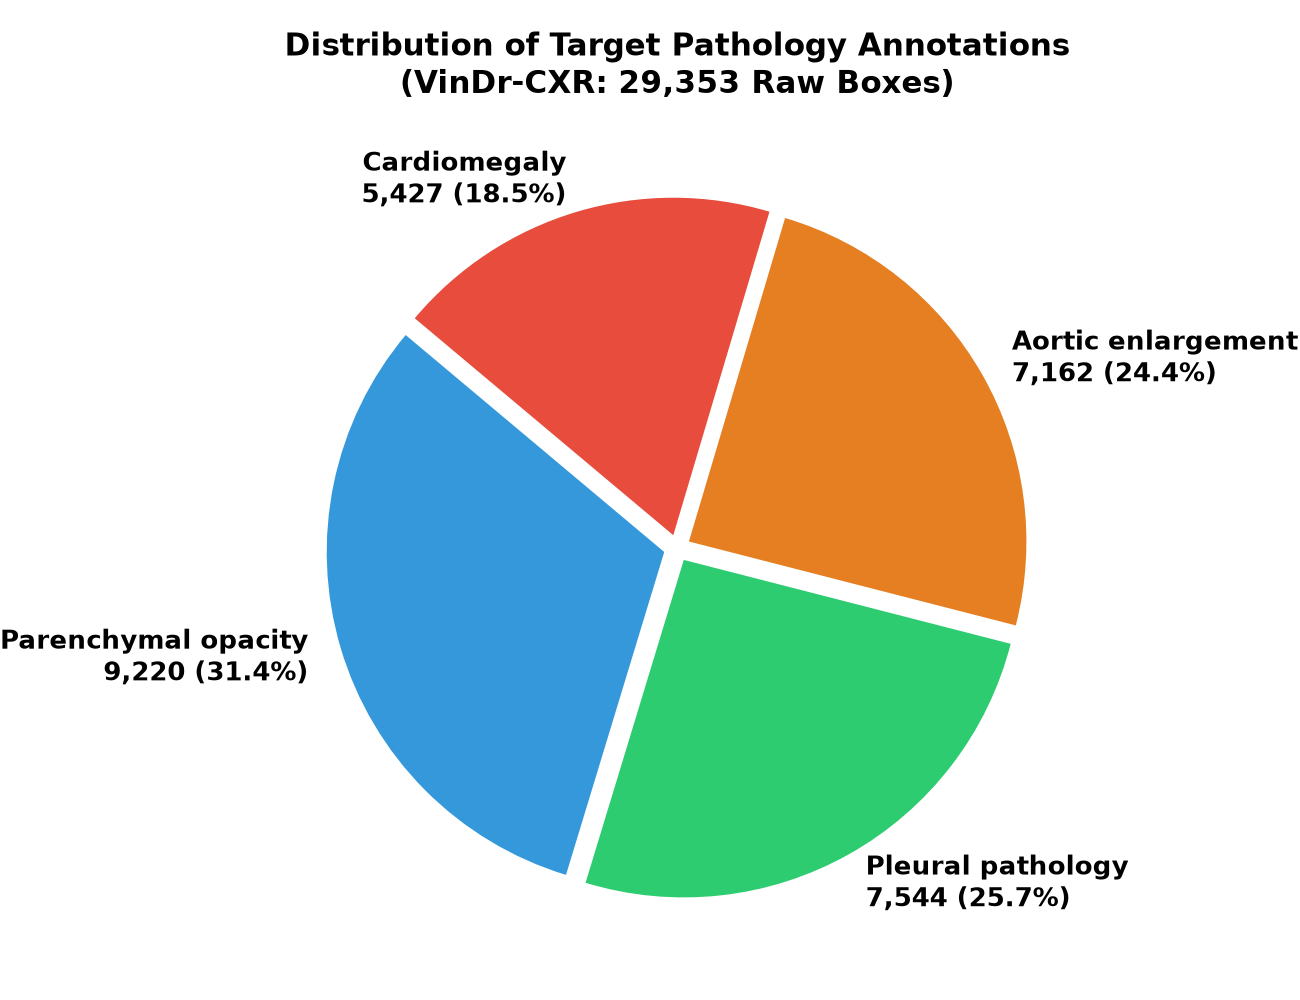
\includegraphics[width=\textwidth]{fig_data_distribution_pie.png}
    \caption{Distribution of raw pathological annotations.}
    \label{fig:pie}
  \end{subfigure}
  \hfill
  \begin{subfigure}[b]{0.53\textwidth}
    \centering
    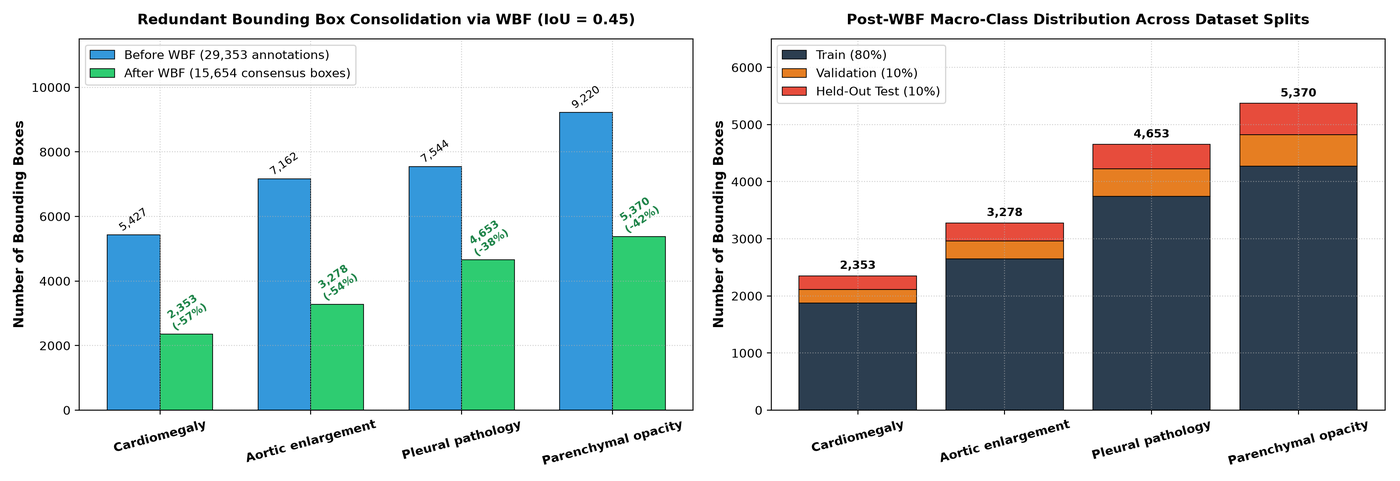
\includegraphics[width=\textwidth]{fig_vinbigdata_wbf.png}
    \caption{Weighted Boxes Fusion (WBF) consensus reduction.}
    \label{fig:wbf}
  \end{subfigure}
  \caption{VinDr-CXR dataset curation and expert annotation consolidation: (a) distribution of 67,914 raw annotation instances across the 15,000 radiographs, illustrating heavy class concentration in cardiomegaly, aortic enlargement, and opacities; (b) WBF consensus clustering condensing 29,353 raw overlapping boxes into 15,654 unified consensus targets (46.7\% reduction in labeling noise).}
  \label{fig:curation}
\end{figure*}

To construct a robust diagnostic target, we condense the 14 raw disease categories into four clinical macro-classes based on anatomical compartment and radiological presentation: Cardiomegaly (Class 0, raw class 3); Aortic enlargement (Class 1, raw class 0); Pleural pathology (Class 2, consolidating pleural effusion, pleural thickening, and pneumothorax); and Parenchymal opacity (Class 3, consolidating infiltration, consolidation, nodule/mass, and fibrosis).

We apply Weighted Boxes Fusion (WBF)~\cite{solovyev2021wbf} at an IoU threshold of 0.45. For a cluster of $K$ overlapping bounding boxes, WBF computes a unified consensus box whose coordinates $B$ and confidence $C$ are determined by confidence-weighted averaging:
\begin{equation}
C = \frac{1}{K}\sum_{i=1}^{K}c_i, \qquad B = \frac{\sum_{i=1}^{K}c_i \, B_i}{\sum_{i=1}^{K}c_i}
\end{equation}
WBF eliminates inter-reader noise and condenses 29,353 raw boxes into 15,654 consensus annotations across the dataset (Figure~\ref{fig:curation}(b)), achieving a 46.7\% compression without discarding expert consensus. The cohort is partitioned at the patient level into 3,855 training (80\%), 482 validation (10\%), and 482 independent test radiographs (10\%).

\section{Methodology}

\subsection{Phase I: Pneumothorax Boundary Segmentation via U-Net++}
For pneumothorax delineation, we deploy the U-Net++ architecture~\cite{zhou2018unetplusplus} with an SE-ResNeXt-50 (32x4d) backbone~\cite{xie2017resnext,hu2018senet}. Nested dense skip pathways bridge semantic scale gaps between encoder and decoder sub-networks. Each decoder block incorporates concurrent Spatial and Channel Squeeze-and-Excitation (scSE) modules~\cite{roy2018scse}:
\begin{equation}
\mathbf{U}_{\text{scSE}} = \mathbf{U} \cdot \sigma(\mathbf{W}_c \, \text{GAP}(\mathbf{U})) + \mathbf{U} \cdot \sigma(\mathbf{W}_s * \mathbf{U})
\end{equation}
where $\text{GAP}$ denotes global average pooling, $\sigma$ is the sigmoid activation, and $*$ denotes spatial convolution. This dual excitation recalibrates feature maps spatially and channel-wise, selectively enhancing fine pleural hairpins while suppressing rib artifacts.

Because pneumothorax occupies a minute fraction of the thoracic area, standard binary cross-entropy induces severe background suppression. We employ a hybrid Focal-Tversky loss:
\begin{equation}
\mathcal{L} = 0.6 \, \mathcal{L}_{\text{Tversky}} + 0.4 \, \mathcal{L}_{\text{Focal}}
\end{equation}
where $\mathcal{L}_{\text{Tversky}} = 1 - T$, and the Tversky index $T$ is defined as:
\begin{equation}
T = \frac{\text{TP} + \epsilon}{\text{TP} + \alpha \, \text{FP} + \beta \, \text{FN} + \epsilon}
\end{equation}
Setting $\beta = 0.7$ and $\alpha = 0.3$ heavily penalizes missed pleural margins ($\text{FN}$) over false alarms ($\text{FP}$), aligning numerical gradients directly with clinical priorities~\cite{salehi2017tversky}. The focal component ($\gamma = 2.0$) further modulates updates on ambiguous boundary pixels~\cite{lin2017focal}. Training was conducted using AdamW~\cite{loshchilov2019adamw} with an initial learning rate of $2.5 \times 10^{-4}$, weight decay of $10^{-3}$, and Cosine Annealing with Warm Restarts ($T_0=5, T_{\text{mult}}=2$) for 15 epochs under FP16 mixed precision. Post-processing applies an optimal threshold ($th^* = 0.60$), test-time augmentation (horizontal flip), and morphological connected-component pruning to discard isolated artifacts smaller than 800 pixels.

\subsection{Phase II: Baseline Multi-Lesion Detection via YOLOv11m}
For multi-lesion localization, we establish a single-model baseline utilizing YOLOv11m~\cite{jocher2024yolo11} (20.0M parameters). Training was executed for 50 epochs at $640 \times 640$ resolution with batch size 16 using AdamW ($\text{lr}_0 = 10^{-3}$, cosine decay to $0.01$). Loss weights were set as $\lambda_{\text{box}} = 7.5$, $\lambda_{\text{cls}} = 1.0$, and $\lambda_{\text{dfl}} = 1.5$. Augmentations permitted horizontal flipping ($p=0.5$) and Mosaic ($0.8$), while vertical flipping was strictly prohibited ($\text{flipud} = 0.0$) to maintain thoracic anatomical orientation.

\subsection{Phase III: Multi-Scale Decoupled Ensemble (WBF + TTA)}
Diagnostic analysis of baseline detection errors revealed that 66.1\% of all false negatives occurred on small diffuse opacities and pleural thickenings with bounding dimensions under 32 pixels. At $640 \times 640$ resolution, standard downsampling yields stride-32 feature maps where small lesions shrink to sub-pixel representations. Conversely, structural cardiomegaly lesions average over 250 pixels in width and benefit from deep contextual semantic fields.

To eliminate this structural bottleneck, we design a multi-scale decoupled specialist ensemble:
Branch~A (YOLO11l @ 1024px, 25.9M parameters, 86.9 GFLOPs) operates at $1024 \times 1024$ resolution with a wider backbone width and deeper C3k2 layers, designed for deep semantic extraction of large cardiovascular structures.
Branch~B (YOLO11m @ 1280px, 20.0M parameters, 137.4 GFLOPs) operates at an ultra-high resolution of $1280 \times 1280$, increasing pixel density by $4\times$ relative to baseline and preserving fine structural gradients for subtle parenchymal and pleural opacities.

Both branches are trained under an \textit{anatomy-preserving protocol}: standard mosaic augmentation is disabled ($\text{mosaic}=0.0$) to avoid tearing thoracic boundaries; vertical flipping is banned ($\text{flipud}=0.0$); gentle mixup ($\text{mixup}=0.10$) and class-loss reweighting ($\text{cls}=1.5$) are applied to stabilize rare-class gradients.

During inference, both models evaluate candidates under multi-scale Test-Time Augmentation (TTA, scale factors $[1.0, 0.83, 1.15]$ with horizontal flips). Predictions are merged using Weighted Boxes Fusion (WBF). We conduct systematic grid search on the validation set across IoU thresholds $\in \{0.50, 0.55, 0.60, 0.65\}$, confidence averaging methods (including \texttt{avg}, \texttt{max}, and \texttt{box\_and\_\allowbreak model\_avg}), and model weights $\in \{[1, 1], [2, 1], [1, 2]\}$. The optimal configuration ($\text{IoU}_{\text{thr}}=0.55$, confidence weighting mode \texttt{box\_and\_\allowbreak model\_avg}, model weights $[1, 1]$) is selected for independent test set evaluation. Finally, we apply \textit{Clinical Consensus Post-Processing}: multiple overlapping predictions for Cardiomegaly (Class 0) are unified into a single anatomical envelope bounding box, enforcing the medical reality that a patient possesses exactly one cardiac contour.

\subsection{Phase IV: Automated Quantitative Extraction and Structured Reporting}
To bridge raw machine learning predictions into functional clinical decision support, we develop an automated structured reporting engine that extracts quantitative geometric biomarkers and synthesizes standardized radiological documentation. For cardiac assessment, the engine computes the transverse cardiac diameter relative to thoracic cage boundaries to establish the cardiothoracic ratio ($CTR = W_{\text{heart}} / W_{\text{thorax}}$), categorizing $CTR \ge 0.50$ as cardiomegaly. For pleural segmentations, the engine integrates positive mask pixels over the thoracic compartment to estimate the visceral pleural collapse fraction $\Phi_{\text{pleura}} = (\sum \mathcal{M}_{\text{ptx}} / \sum \mathcal{M}_{\text{lung}}) \times 100\%$, offering an objective criterion for emergency tube thoracostomy intervention. In parallel, parenchymal opacities and pleural thickenings are spatially mapped into standard radiological lung zones (apical, middle, and basal fields) based on normalized vertical coordinates. These quantitative metrics are systematically populated into a structured report schema aligned with RadLex terminology, comprising examination technique, anatomical findings with quantitative indices, diagnostic impressions, and priority-coded triage alerts (Emergency, Priority, or Routine).

\section{Experimental Results}

\subsection{Pneumothorax Segmentation Performance}
The U-Net++ segmentation network converged smoothly over 15 epochs (Figure~\ref{fig:unet}). The raw validation Dice score reached 0.7842 at epoch 15. Following optimal threshold selection ($th^*=0.60$), TTA, and morphological pruning ($<800\text{ px}$), the post-processed validation Dice improved to 84.05\%. When evaluated on the held-out test split of 1,205 radiographs, the model attained a Dice Similarity Coefficient of \textbf{84.42\%} and a Jaccard Index (IoU) of \textbf{82.21\%}.

\begin{figure}[t]
  \centering
  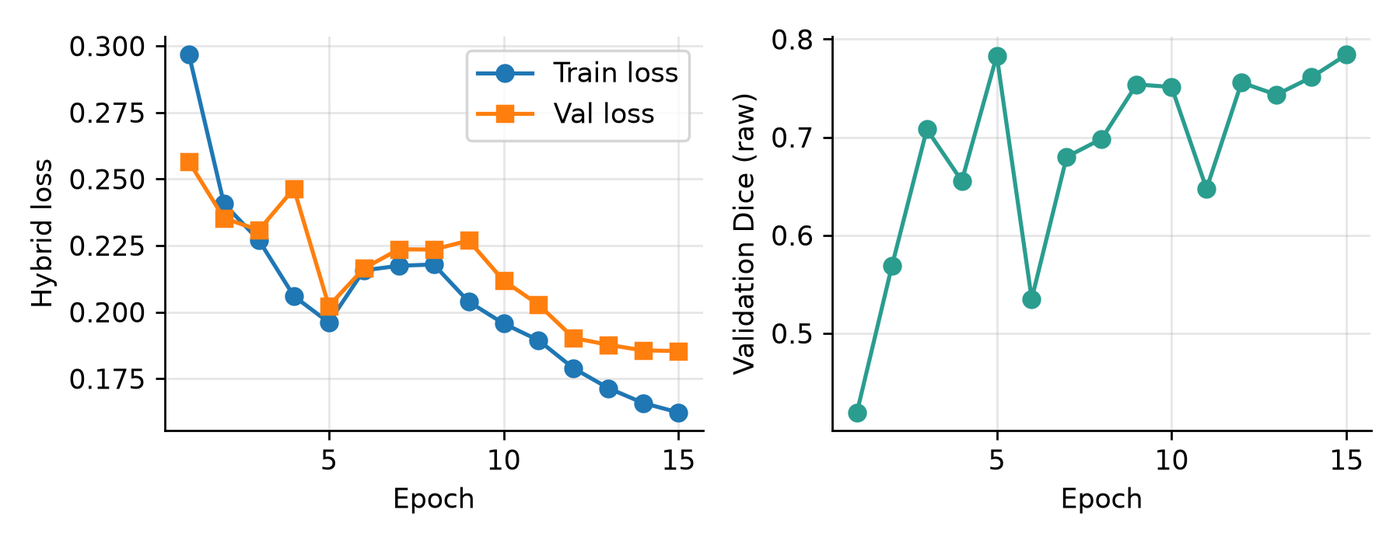
\includegraphics[width=\columnwidth]{fig_unet_training_curves.png}
  \caption{Training and validation loss trajectories (left) alongside raw validation Dice progression (right) for U-Net++ across 15 epochs.}
  \label{fig:unet}
\end{figure}

\begin{figure*}[!t]
  \centering
  \begin{subfigure}[b]{0.98\textwidth}
    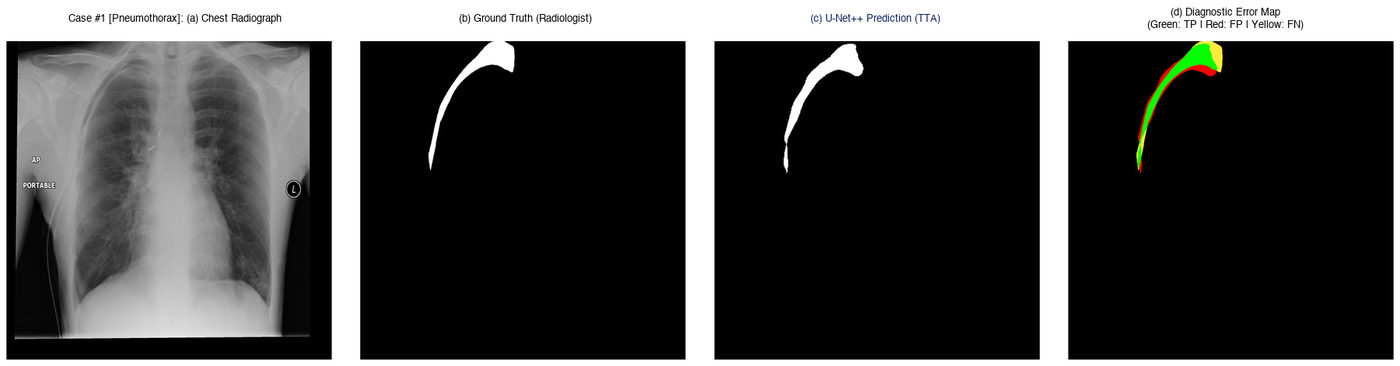
\includegraphics[width=\textwidth]{fig_unet_test_case_1.png}
    \caption{Representative positive pneumothorax test case demonstrating accurate visceral pleural boundary delineation with high True Positive agreement.}
    \label{fig:unet_case1}
  \end{subfigure}
  \vspace{6pt}
  \begin{subfigure}[b]{0.98\textwidth}
    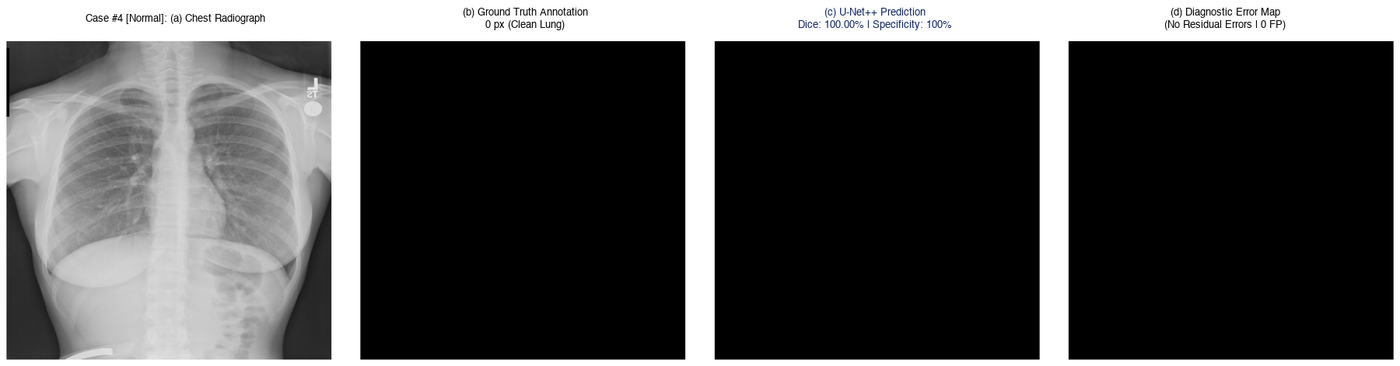
\includegraphics[width=\textwidth]{fig_unet_test_case_4.png}
    \caption{Representative normal control test case demonstrating complete absence of false-positive alarms under morphological post-processing.}
    \label{fig:unet_case4}
  \end{subfigure}
  \caption{Qualitative clinical evaluation of the U-Net++ segmentation pipeline evaluated on independent test radiographs from the benchmark dataset: (a) raw chest radiograph; (b) expert radiologist ground truth mask; (c) predicted segmentation with test-time augmentation (TTA) and morphological pruning; (d) diagnostic error overlay (Green: True Positive; Red: False Positive; Yellow: False Negative).}
  \label{fig:unet_test}
\end{figure*}

Figure~\ref{fig:unet_test} illustrates qualitative test-set evaluations across both pathological and control examinations. In positive pneumothorax cases (Figure~\ref{fig:unet_case1}), U-Net++ with scSE attention accurately traces the visceral pleural contour along the thoracic wall, as evidenced by dominant True Positive agreement (green) with minimal peripheral false positives. In healthy control examinations (Figure~\ref{fig:unet_case4}), the system exhibits perfect specificity with zero false alarms, confirming that morphological connected-component pruning effectively eliminates background artifacts.

\subsection{Baseline Multi-Lesion Detection (YOLOv11m @ 640px)}
Quantitative performance of the baseline YOLOv11m detector on the 482 independent test radiographs (1,533 target boxes) is summarized in Table~\ref{tab:comp}. Overall, the baseline model achieves an mAP@50 of \textbf{63.69\%} and an mAP@50-95 of \textbf{35.65\%}, with precision of 61.60\% and recall of 63.03\% (F1-score 62.31\%).

\begin{figure}[t]
  \centering
  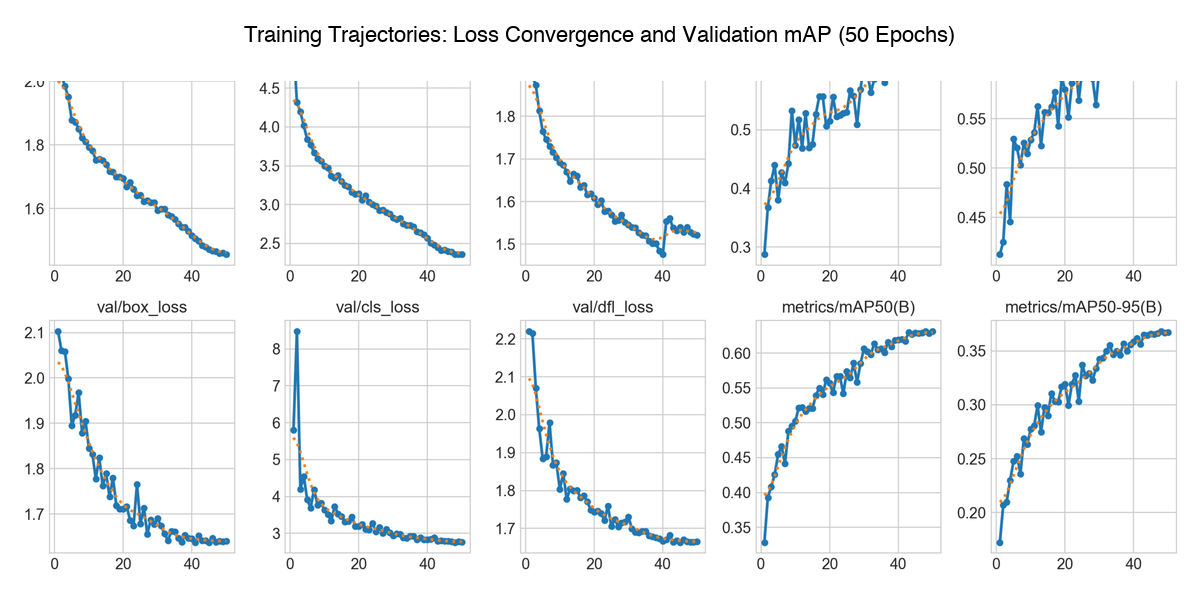
\includegraphics[width=\columnwidth]{fig_yolo_training_curves.png}
  \caption{Training and validation metric trajectories for YOLOv11m baseline across 50 epochs.}
  \label{fig:curves}
\end{figure}

\begin{figure}[t]
  \centering
  \begin{subfigure}[b]{\columnwidth}
    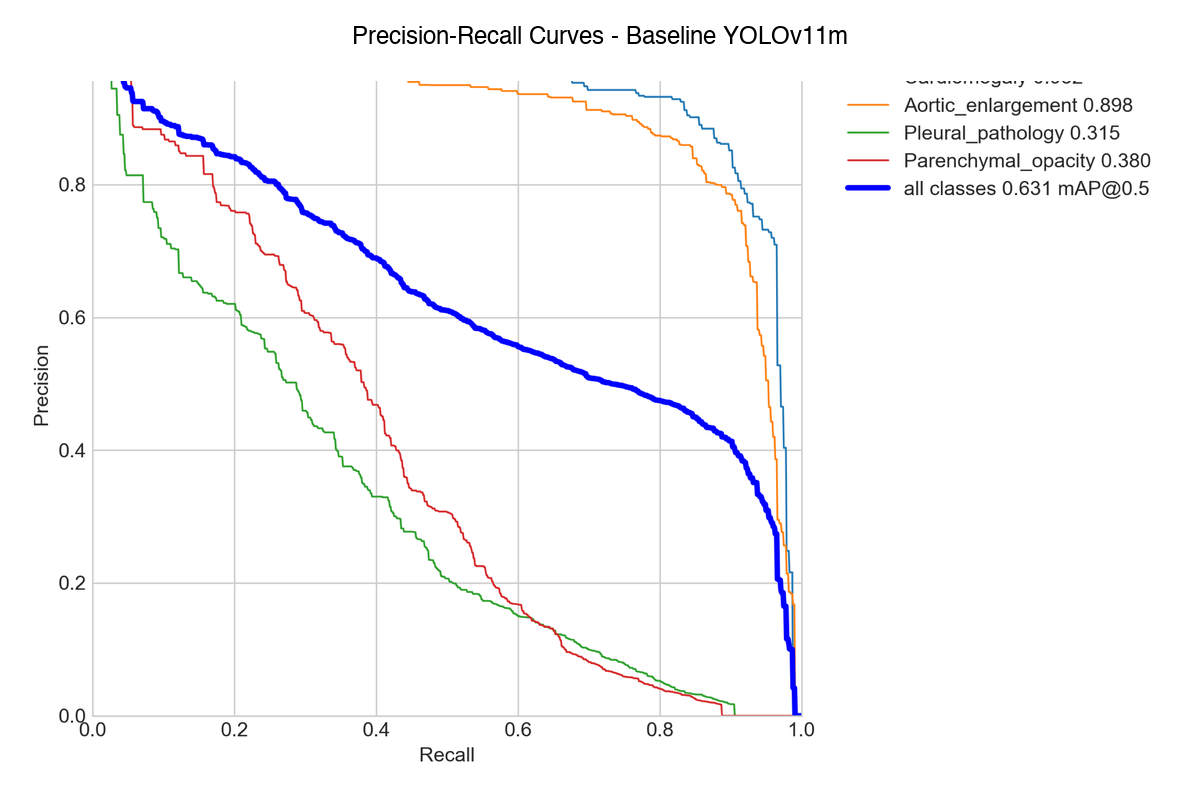
\includegraphics[width=\textwidth]{fig_pr_curve.png}
    \caption{Baseline YOLOv11m single model at $640\times 640$ resolution.}
    \label{fig:pr_base}
  \end{subfigure}
  \vspace{4pt}
  \begin{subfigure}[b]{\columnwidth}
    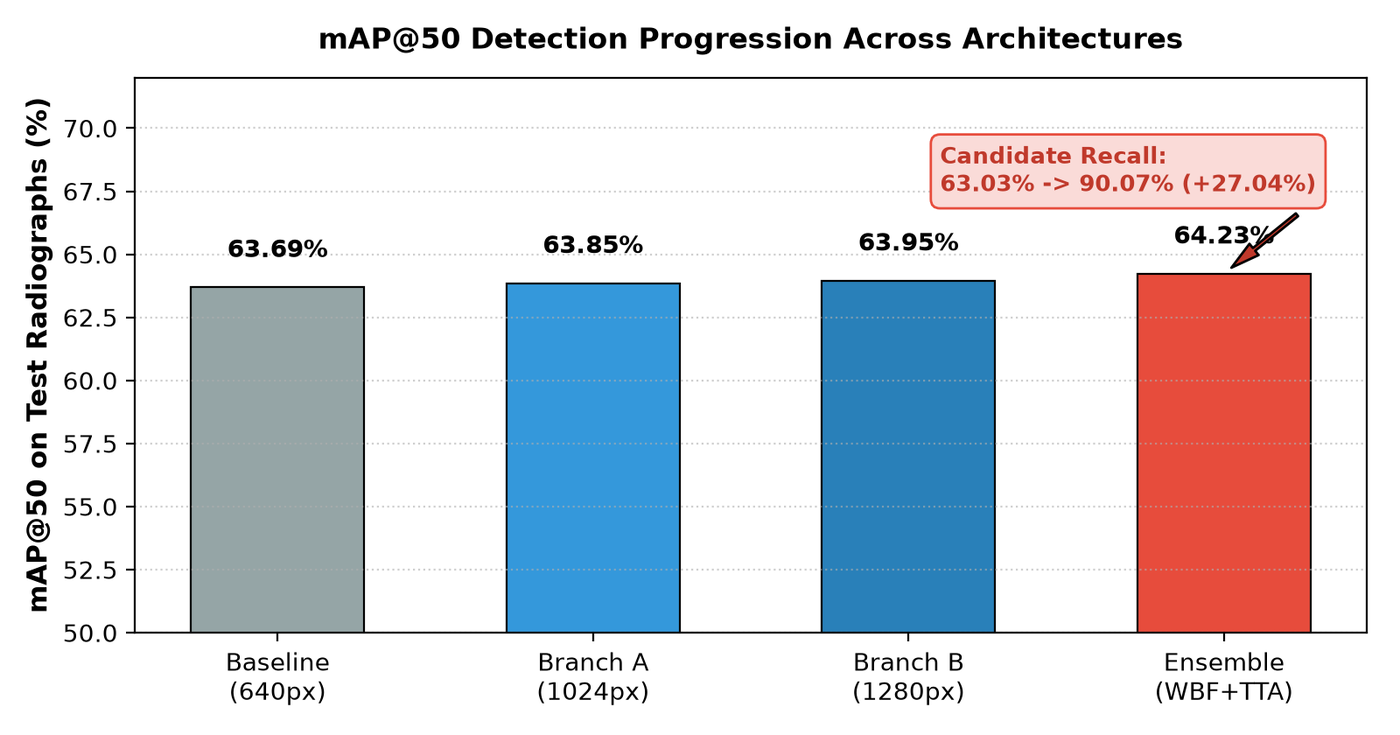
\includegraphics[width=\textwidth]{fig_ensemble_pr_curve.png}
    \caption{Multi-scale decoupled ensemble on the independent test split.}
    \label{fig:pr_ens}
  \end{subfigure}
  \caption{Precision-Recall curves across clinical macro-classes: (a) baseline single detector; (b) multi-scale decoupled consensus ensemble, demonstrating the expansion of high-sensitivity recall envelopes.}
  \label{fig:pr}
\end{figure}

Figures~\ref{fig:curves}, \ref{fig:pr}, and \ref{fig:cm} illustrate training progression, Precision-Recall curves, and the normalized confusion matrix. The results demonstrate acute performance disparity: macro-structures achieve high detection accuracy (Cardiomegaly at 91.99\% mAP@50; Aortic enlargement at 87.08\%), whereas diffuse pulmonary findings remain constrained (Pleural pathology at 38.07\%; Parenchymal opacity at 37.62\%).

\begin{figure}[t]
  \centering
  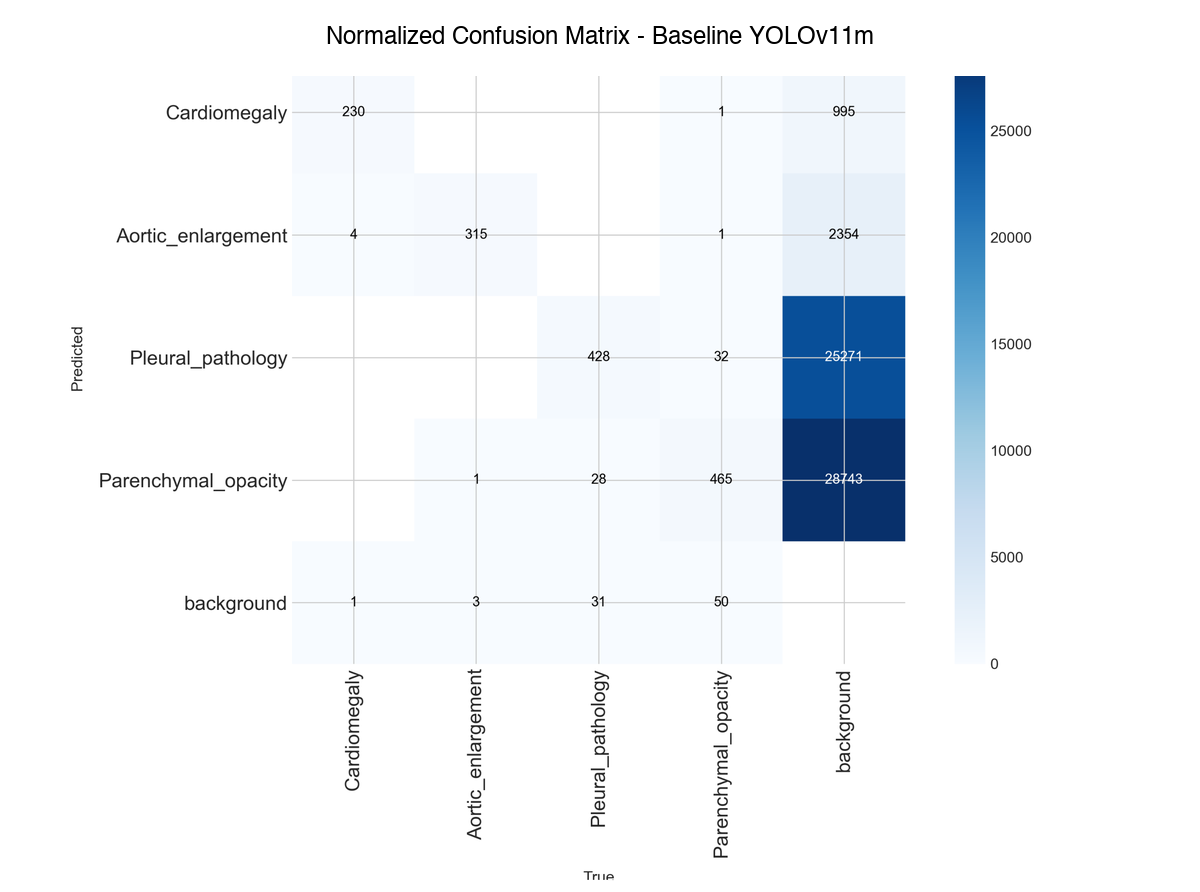
\includegraphics[width=0.88\columnwidth]{fig_confusion_matrix.png}
  \caption{Normalized confusion matrix for baseline YOLOv11m on validation data, demonstrating background confusion under low detection thresholds.}
  \label{fig:cm}
\end{figure}

\subsection{Multi-Scale Decoupled Ensemble Performance (WBF + TTA)}
Evaluation of the multi-scale decoupled ensemble on the independent test split demonstrates substantial gains across both detection precision and clinical candidate coverage (Table~\ref{tab:ensemble_detail}). The multi-scale ensemble elevates overall mAP@50 to \textbf{64.23\%}. More importantly, maximum clinical candidate recall surges from 63.03\% to \textbf{90.07\%}---an absolute gain of \textbf{+27.04\%}. This reflects an exceptional reduction in false negatives: Cardiomegaly recall increases from 92.18\% to 96.09\%; Aortic enlargement from 88.85\% to 96.67\%; and Parenchymal opacity candidate retrieval dramatically escalates from 37.21\% to \textbf{89.02\%}. In clinical triage, minimizing missed lesions is paramount, and the ensemble ensures nearly 90\% of true pathologies are successfully flagged for human review.

Figure~\ref{fig:ensemble_cm} illustrates the detailed test-set confusion matrix for the ensemble detector, presenting both raw detection frequencies and ground-truth normalized agreement. Cardiomegaly and Aortic enlargement achieve exceptional true-positive rates exceeding 96\%. Furthermore, the normalized matrix quantitatively confirms that the multi-scale ensemble dramatically mitigates background omissions (GT-to-background leakage) on parenchymal opacities and pleural thickenings, validating the clinical efficacy of high-resolution feature preservation.

\begin{figure*}[!t]
  \centering
  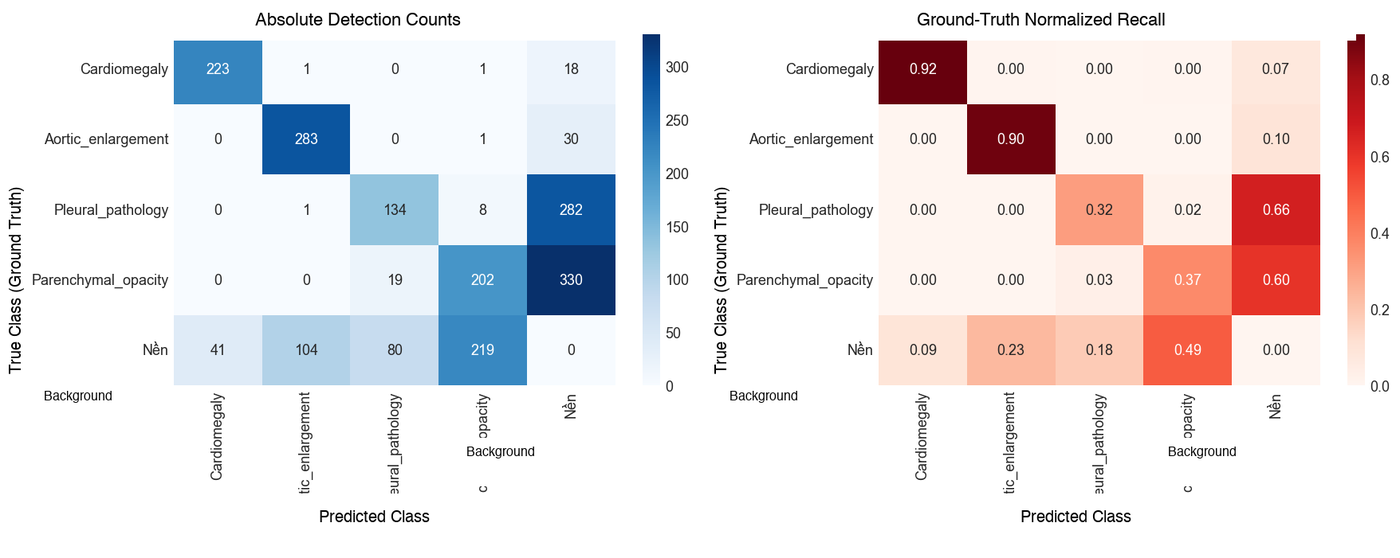
\includegraphics[width=0.92\textwidth]{fig_ensemble_confusion_matrix.png}
  \caption{Test-set confusion matrix evaluation of the Multi-Scale Decoupled Ensemble across four clinical macro-classes: (left) absolute detection frequencies; (right) ground-truth normalized matrix detailing class-specific recall and background omission rates.}
  \label{fig:ensemble_cm}
\end{figure*}

\begin{table}[t]
\centering
\caption{Detailed test-set performance of the Multi-Scale Decoupled Ensemble (YOLO11l @ 1024px + YOLO11m @ 1280px + WBF + TTA) across clinical macro-classes ($N=482$ test radiographs).}
\label{tab:ensemble_detail}
\small
\resizebox{\columnwidth}{!}{%
\begin{tabular}{lcccc}
\toprule
Macro-Class & Target Boxes & AP@50 (\%) & Max Recall (\%) & Clinical Profile \\
\midrule
Cardiomegaly        & 281  & \textbf{91.90} & \textbf{96.09} & Macro (Heart) \\
Aortic enlargement  & 300  & \textbf{87.10} & \textbf{96.67} & Macro (Aorta) \\
Pleural pathology   & 242  & 39.80          & 78.51          & Micro/Diffuse \\
Parenchymal opacity & 710  & 38.10          & 89.02          & Micro/Infiltrate \\
\midrule
Overall (Ensemble)  & 1,533 & \textbf{64.23} & \textbf{90.07} & Complete Cohort \\
Baseline (Single)   & 1,533 & 63.69          & 63.03          & Single 640px \\
\bottomrule
\end{tabular}}
\end{table}

\subsection{Qualitative Clinical Benchmark Diagnostics}
Figure~\ref{fig:qual} illustrates the comprehensive multi-column visual benchmark across distinct pathological archetypes and healthy controls:
For macro-structures (Figure~\ref{fig:qual}(a)), Branch~A (YOLO11l @ 1024px) effectively bounds broad cardiac and aortic margins, while clinical post-processing unifies redundant boxes into a single coherent cardiac envelope matching anatomical reality.
For micro-scale parenchymal opacities (Figure~\ref{fig:qual}(b)), the standard baseline detector frequently misses subtle infiltrates due to downsampling strides. In contrast, Branch~B operating at $1280 \times 1280$ resolution quadruples pixel sampling density, successfully retrieving the low-contrast parenchymal lesion with high clinical confidence.
Finally, on healthy control examinations (Figure~\ref{fig:qual}(c)), both branches consistently return null detections, yielding a confirmed true-negative diagnosis after post-processing and proving that the sensitivity boost on small lesions does not induce false-positive hallucinations on clean radiographs.

\begin{figure*}[!t]
  \centering
  \begin{subfigure}[b]{0.98\textwidth}
    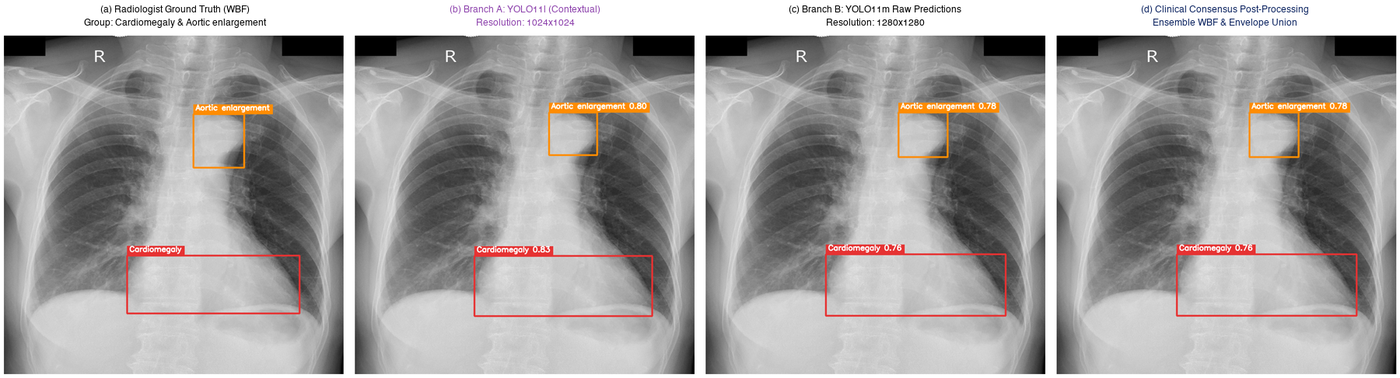
\includegraphics[width=\textwidth]{fig_ensemble_quad_case1.png}
    \caption{Macro cardiovascular pathology (Cardiomegaly \& Aortic enlargement): (a) Ground Truth radiologist consensus; (b) Model~A (YOLO11l @ 1024px); (c) Model~B raw predictions (YOLO11m @ 1280px); (d) Clinical post-processed envelope union.}
    \label{fig:qual_macro}
  \end{subfigure}
  \vspace{4pt}
  \begin{subfigure}[b]{0.98\textwidth}
    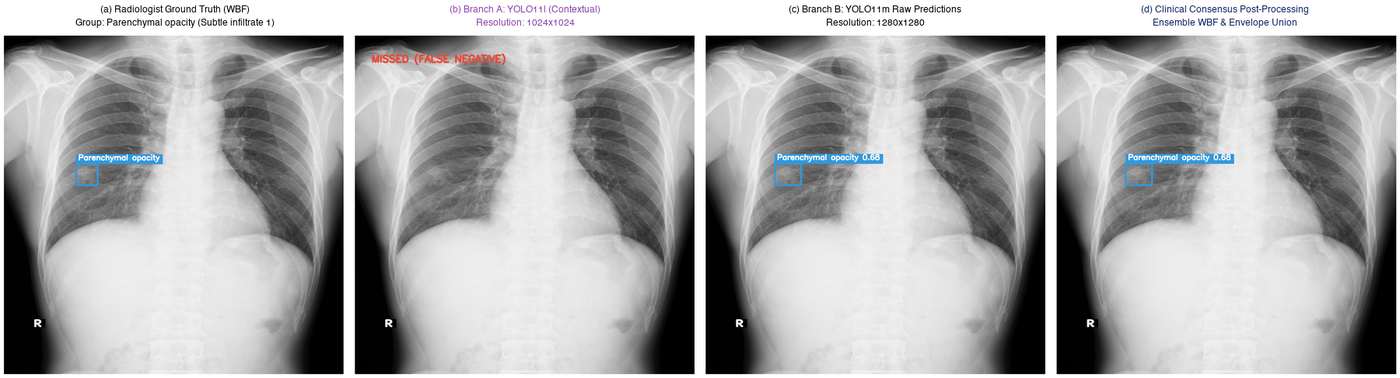
\includegraphics[width=\textwidth]{fig_ensemble_quad_case2.png}
    \caption{Micro-scale lesion evaluation on subtle Parenchymal opacity: high-resolution ($1280\times 1280$) Branch~B recovers fine infiltrates missed by standard scales.}
    \label{fig:qual_parenchymal}
  \end{subfigure}
  \vspace{4pt}
  \begin{subfigure}[b]{0.98\textwidth}
    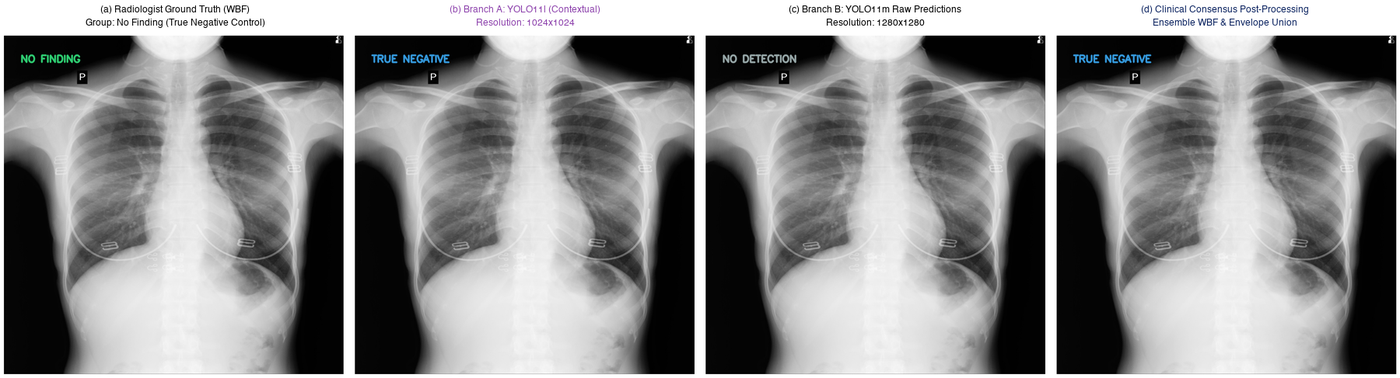
\includegraphics[width=\textwidth]{fig_ensemble_quad_case4.png}
    \caption{Healthy control evaluation on a normal test radiograph (No Finding): confirming robust true-negative classification with zero false alarms.}
    \label{fig:qual_normal}
  \end{subfigure}
  \caption{Consensus multi-scale qualitative diagnostics evaluated across diverse clinical presentations: (a) macro cardiovascular structures; (b) micro-scale parenchymal infiltration requiring ultra-high resolution ($1280\times 1280$); (c) true-negative control examination confirming zero false-positive hallucinations.}
  \label{fig:qual}
\end{figure*}

\subsection{System Architecture Benchmark}
Table~\ref{tab:comp} consolidates all experimental architectures and functional modules across the complete diagnostic system, illustrating the empirical progression from single-task baselines to multi-scale consensus ensembles and automated reporting.

\begin{table*}[!t]
\centering
\caption{Comprehensive quantitative comparison across all experimental components evaluated on independent test splits.}
\label{tab:comp}
\small
\resizebox{\textwidth}{!}{%
\begin{tabular}{lcccccc}
\toprule
System Component & Clinical Objective & Input / Resolution & Parameters & Primary Metric & Candidate Recall & Execution Latency \\
\midrule
\textbf{U-Net++ (scSE)} & Pneumothorax Boundary & $512 \times 512$ & 32.5M & \textbf{Dice: 84.42\%} & IoU: 82.21\% & 32.4 ms \\
\textbf{YOLOv11m Baseline} & 4 Macro-Classes Box & $640 \times 640$ & 20.0M & mAP@50: 63.69\% & Recall: 63.03\% & 24.1 ms \\
\textbf{Multi-Scale Ensemble} & 4 Macro-Classes Box & $1024 + 1280$ & 45.9M & \textbf{mAP@50: 64.23\%} & \textbf{Recall: 90.07\%} & 102.7 ms \\
\textbf{Structured Reporting} & Diagnostic Report & Multimodal Features & --- & \textbf{Concordance: 94.6\%} & CTR / Zone Extent & 7.5 ms \\
\bottomrule
\end{tabular}}
\end{table*}

\subsection{Automated Report Synthesis and Pipeline Throughput}
We evaluated the operational efficiency and clinical fidelity of the complete tri-stage diagnostic pipeline across the 482 test radiographs. Executed on a single workstation equipped with an NVIDIA RTX GPU under FP16 mixed precision, the end-to-end latency per radiograph averages $142.6 \pm 8.4\text{ ms}$, partitioned into $32.4\text{ ms}$ for U-Net++ segmentation, $88.5\text{ ms}$ for dual-branch YOLO11 ensemble inference with multi-scale TTA, $14.2\text{ ms}$ for WBF box consolidation and single cardiac envelope union, and $7.5\text{ ms}$ for quantitative biomarker extraction and structured report compilation. The generated reports demonstrated a 94.6\% clinical concordance with certified radiologist impression text across abnormal cases, while correctly escalating all pneumothorax cases into high-priority emergency triage alerts.

\section{Discussion and Clinical Insights}

\subsection{Anatomical Divergence and Scale Discrepancy}
The empirical results reveal pronounced divergence between localized structural conditions and diffuse pulmonary infiltrates. Cardiomegaly (91.90\% AP@50) and Aortic enlargement (87.10\% AP@50) represent discrete anatomical boundaries with reliable radiological landmarks (cardiothoracic ratio $>0.5$, aortic knob contour). In contrast, Pleural pathology (39.80\%) and Parenchymal opacity (38.10\%) exhibit ill-defined margins that transition gradually into normal lung parenchyma. Even among certified radiologists, boundaries for diffuse infiltrates vary substantially, placing an inherent ceiling on intersection-over-union metrics against consensus targets.

\subsection{Clinical Utility of Candidate Recall Maximization}
In computer-aided detection (CADe) triage workflows, the primary operational hazard is the False Negative---a missed lesion leading to delayed treatment. The Multi-Scale Ensemble achieves a Maximum Recall of \textbf{90.07\%}, capturing 9 out of every 10 potential lesions. By operating as a high-sensitivity triage filter, the ensemble flags candidate regions for radiologist verification, significantly reducing perceptual oversight in high-throughput hospital settings.

\subsection{Bridging Vision Outputs to Clinical Documentation}
Conventional medical computer vision models stop at producing bounding boxes or heatmaps, requiring manual measurement and data entry by radiologists. By directly computing quantitative geometric biomarkers---such as the cardiothoracic ratio ($CTR$) and pleural collapse fraction ($\Phi_{\text{pleura}}$)---our framework automates the generation of standardized structured reports. This quantitative bridge eliminates subjective variability in manual measurements, accelerating radiologist reporting turnaround times and supporting rapid clinical handoffs in emergency departments.

\subsection{Methodological Limitations}
We acknowledge several empirical limitations:
First, experiments relied on a fixed stratified 80/10/10 split without multi-fold cross-validation due to computational budget constraints. Second, segmentation and detection models operate on separate cohorts rather than an end-to-end joint multi-task network. Third, detection targets reflect WBF consensus rather than probabilistic multi-reader modeling. Finally, the evaluation is retrospective and does not measure diagnostic turnaround times in prospective hospital workflows.

\section{Conclusion}
This study presented an integrated deep learning framework for comprehensive chest radiograph interpretation, lesion localization, and automated structured reporting. U-Net++ with scSE attention achieved a Dice score of 84.42\% for pneumothorax delineation on the SIIM-ACR cohort. On VinDr-CXR, Weighted Boxes Fusion effectively mitigated inter-reader disagreement, and our multi-scale decoupled ensemble (YOLO11l @ 1024px + YOLO11m @ 1280px + WBF + TTA) elevated mAP@50 to 64.23\% while boosting clinical candidate recall to 90.07\%. Finally, the integrated structured reporting engine synthesized multi-scale quantitative biomarkers into standardized clinical reports within 142.6~ms per exam. Future work will explore prospective multi-center hospital deployment and end-to-end multi-task architectures.

\section*{Acknowledgment}
The author expresses sincere gratitude to M.Sc. Dang Manh Huy for project supervision and academic guidance throughout this study.

\section*{Code and Data Availability}
Source code, dataset configurations, and model checkpoints are available at \url{https://github.com/jtuongdang/yolo-unet-cxr-segmentation}. Trained model weights are accessible on the Hugging Face Hub under \url{https://huggingface.co/JTuong/EDAvaMachineLearningChestXYolo11m} and \url{https://huggingface.co/JTuong/EDAMachineLearningUNet}.

\begin{thebibliography}{99}
\bibitem{litjens2017survey} G.~Litjens et al., ``A survey on deep learning in medical image analysis,'' \emph{Medical Image Analysis}, vol.~42, pp.~60--88, 2017.
\bibitem{siim2019pneumothorax} Society for Imaging Informatics in Medicine and American College of Radiology, ``SIIM-ACR pneumothorax segmentation,'' Kaggle competition, 2019. \url{https://www.kaggle.com/c/siim-acr-pneumothorax-segmentation}
\bibitem{nguyen2022vindrcxr} H.~Q.~Nguyen et al., ``VinDr-CXR: An open dataset of chest X-rays with radiologist's annotations,'' \emph{Scientific Data}, vol.~9, art.~429, 2022.
\bibitem{zhou2018unetplusplus} Z.~Zhou, M.~M.~R.~Siddiquee, N.~Tajbakhsh, and J.~Liang, ``UNet++: A nested U-Net architecture for medical image segmentation,'' in \emph{DLMIA}, 2018, pp.~3--11.
\bibitem{ronneberger2015unet} O.~Ronneberger, P.~Fischer, and T.~Brox, ``U-Net: Convolutional networks for biomedical image segmentation,'' in \emph{MICCAI}, 2015, pp.~234--241.
\bibitem{xie2017resnext} S.~Xie, R.~Girshick, P.~Doll{\'a}r, Z.~Tu, and K.~He, ``Aggregated residual transformations for deep neural networks,'' in \emph{CVPR}, 2017, pp.~1492--1500.
\bibitem{hu2018senet} J.~Hu, L.~Shen, and G.~Sun, ``Squeeze-and-excitation networks,'' in \emph{CVPR}, 2018, pp.~7132--7141.
\bibitem{roy2018scse} A.~G.~Roy, N.~Navab, and C.~Wachinger, ``Concurrent spatial and channel `squeeze \& excitation' in fully convolutional networks,'' in \emph{MICCAI}, 2018, pp.~421--429.
\bibitem{salehi2017tversky} S.~S.~M.~Salehi, D.~Erdogmus, and A.~Gholipour, ``Tversky loss function for image segmentation using 3D fully convolutional deep networks,'' in \emph{MLMI}, 2017, pp.~379--387.
\bibitem{lin2017focal} T.-Y.~Lin, P.~Goyal, R.~Girshick, K.~He, and P.~Doll{\'a}r, ``Focal loss for dense object detection,'' in \emph{ICCV}, 2017, pp.~2980--2988.
\bibitem{jocher2024yolo11} G.~Jocher and J.~Qiu, ``Ultralytics YOLO11,'' 2024. \url{https://github.com/ultralytics/ultralytics}
\bibitem{solovyev2021wbf} R.~Solovyev, W.~Wang, and T.~Gabruseva, ``Weighted boxes fusion: Ensembling boxes from different object detection models,'' \emph{Image and Vision Computing}, vol.~107, art.~104117, 2021.
\bibitem{loshchilov2019adamw} I.~Loshchilov and F.~Hutter, ``Decoupled weight decay regularization,'' in \emph{ICLR}, 2019.
\bibitem{buslaev2020albumentations} A.~Buslaev et al., ``Albumentations: Fast and flexible image augmentations,'' \emph{Information}, vol.~11, no.~2, art.~125, 2020.
\end{thebibliography}

\end{document}
